% This is "sig-alternate.tex" V2.0 May 2012
% This file should be compiled with V2.5 of "sig-alternate.cls" May 2012
%
% This example file demonstrates the use of the 'sig-alternate.cls'
% V2.5 LaTeX2e document class file. It is for those submitting
% articles to ACM Conference Proceedings WHO DO NOT WISH TO
% STRICTLY ADHERE TO THE SIGS (PUBS-BOARD-ENDORSED) STYLE.
% The 'sig-alternate.cls' file will produce a similar-looking,
% albeit, 'tighter' paper resulting in, invariably, fewer pages.
%
% ----------------------------------------------------------------------------------------------------------------
% This .tex file (and associated .cls V2.5) produces:
%       1) The Permission Statement
%       2) The Conference (location) Info information
%       3) The Copyright Line with ACM data
%       4) NO page numbers
%
% as against the acm_proc_article-sp.cls file which
% DOES NOT produce 1) thru' 3) above.
%
% Using 'sig-alternate.cls' you have control, however, from within
% the source .tex file, over both the CopyrightYear
% (defaulted to 200X) and the ACM Copyright Data
% (defaulted to X-XXXXX-XX-X/XX/XX).
% e.g.
% \CopyrightYear{2007} will cause 2007 to appear in the copyright line.
% \crdata{0-12345-67-8/90/12} will cause 0-12345-67-8/90/12 to appear in the copyright line.
%
% ---------------------------------------------------------------------------------------------------------------
% This .tex source is an example which *does* use
% the .bib file (from which the .bbl file % is produced).
% REMEMBER HOWEVER: After having produced the .bbl file,
% and prior to final submission, you *NEED* to 'insert'
% your .bbl file into your source .tex file so as to provide
% ONE 'self-contained' source file.
%
% ================= IF YOU HAVE QUESTIONS =======================
% Questions regarding the SIGS styles, SIGS policies and
% procedures, Conferences etc. should be sent to
% Adrienne Griscti (griscti@acm.org)
%
% Technical questions _only_ to
% Gerald Murray (murray@hq.acm.org)
% ===============================================================
%
% For tracking purposes - this is V2.0 - May 2012

\documentclass{sig-alternate}
\usepackage{graphicx}
\usepackage{caption}
\usepackage{subcaption}
\usepackage{multirow}
\usepackage{enumitem}
\usepackage[]{algorithm2e}


\begin{document}
%
% --- Author Metadata here ---
\conferenceinfo{CSC2525}{'14 UofT, CA}
%\CopyrightYear{2007} % Allows default copyright year (20XX) to be over-ridden - IF NEED BE.
%\crdata{0-12345-67-8/90/01}  % Allows default copyright data (0-89791-88-6/97/05) to be over-ridden - IF NEED BE.
% --- End of Author Metadata ---

\title{REACH: Enabling Single-Handed Operation on Large Screen Mobile Devices}

%
% You need the command \numberofauthors to handle the 'placement
% and alignment' of the authors beneath the title.
%
% For aesthetic reasons, we recommend 'three authors at a time'
% i.e. three 'name/affiliation blocks' be placed beneath the title.
%
% NOTE: You are NOT restricted in how many 'rows' of
% "name/affiliations" may appear. We just ask that you restrict
% the number of 'columns' to three.
%
% Because of the available 'opening page real-estate'
% we ask you to refrain from putting more than six authors
% (two rows with three columns) beneath the article title.
% More than six makes the first-page appear very cluttered indeed.
%
% Use the \alignauthor commands to handle the names
% and affiliations for an 'aesthetic maximum' of six authors.
% Add names, affiliations, addresses for
% the seventh etc. author(s) as the argument for the
% \additionalauthors command.
% These 'additional authors' will be output/set for you
% without further effort on your part as the last section in
% the body of your article BEFORE References or any Appendices.

\numberofauthors{3} %  in this sample file, there are a *total*
% of EIGHT authors. SIX appear on the 'first-page' (for formatting
% reasons) and the remaining two appear in the \additionalauthors section.
%
\author{
% You can go ahead and credit any number of authors here,
% e.g. one 'row of three' or two rows (consisting of one row of three
% and a second row of one, two or three).
%
% The command \alignauthor (no curly braces needed) should
% precede each author name, affiliation/snail-mail address and
% e-mail address. Additionally, tag each line of
% affiliation/address with \affaddr, and tag the
% e-mail address with \email.
%
% 1st. author
% 1st. author
\alignauthor
Varun Perumal\\
       \affaddr{Dept. of Computer Science}\\
       \affaddr{University of Toronto}\\
       \email{varun@cs.toronto.edu}
% 2nd author
\alignauthor
Ahmadul Hassan\\
       \affaddr{Elec. \& Computer Eng.}\\
       \affaddr{University of Toronto}\\
       \email{ahmadul.hassan@gmail.com}
% 3rd author
\alignauthor
Zahid Abul-Basher\\
       \affaddr{Mech. \& Industrial Eng.}\\
       \affaddr{University of Toronto}\\
       \email{zahid@cs.toronto.edu}
}
% There's nothing stopping you putting the seventh, eighth, etc.
% author on the opening page (as the 'third row') but we ask,
% for aesthetic reasons that you place these 'additional authors'
% in the \additional authors block, viz.

% Just remember to make sure that the TOTAL number of authors
% is the number that will appear on the first page PLUS the
% number that will appear in the \additionalauthors section.

\maketitle
\begin{abstract}

\end{abstract}

% A category with the (minimum) three required fields
\category{H.5.2}{Information interfaces and presentation}{User Interfaces---graphical user interfaces}
%A category including the fourth, optional field follows...
%\category{D.2.8}{Software Engineering}{Metrics}[complexity measures, performance measures]

\terms{Design, Experimentation, Human Factors}

\keywords{Data analytics}


%=============================================================================
% CONTENT
%=============================================================================

\section{Introduction}
While the rising popularity and adoption of large screen mobile phones presents users with a larger canvas for content consumption, it also poses several significant usability issues. The most important one being the ergonomic mismatch that these larger devices pose for single-handed use. Most of today's mobile interactions are centered on quick, short and intermittent usage patterns. Hence, single-handed interaction with mobile devices is of importance, since it supports these kinds of usage patterns. All device manufacturers who make large screen mobile devices have implemented ways to enable single-handed use. Apple's larger phones allow the user to double tap the home button to quickly pull the entire interface closer to the bottom edge of the screen, Samsung, allows users to snap windows to different corners of the screen to allow for one handed access. However, these methods add an extra step that the user must go through in order to interact with the device, thus breaking the continuity of the interaction.
\par
With REACH we propose to solve the above mentioned problem by appending sensor systems to the phone which can detect when the user is trying to reach the far corners of the phone and affect changes in the UI accordingly. As a bonus, project reach also explores the use of this appended sensor framework to enable additional interaction on mobile devices. Although prior work has been done on sensing grip, our project aims to use this information for a very specific purpose. 			% Introduction
\section{Related Work}
Many researchers have suggested that the devices should be intelligent enough to detect user's situation for better support as in \cite{Johnson:1998:UMIM} and \cite{Schmidt:1999:AIC}. For instance, \emph{ability based design} aims to find the best match between the ability of the users and the interfaces \cite{Wobbrock:2011:adcpe}. There are also researches to recognize the activity of users on devices (also known as \emph{activity recognition}). Choudhuri \emph{et al.} \cite{Choudhury:2008:MSP} built a wearable device with sensors to detect the activity of the users. In \cite{Van:2000:WhatShallWe}, Laerhoven used an accelerometer in a phone to recognize different motions of walking, climbing stairs, \emph{etc}. Schmidt \emph{et al.} \cite{Schmidt:1999:AIC} also used accelerometer but to detect both the user movement and the place of the device itself whether it is in the hand or on a table or in a suitcase. GripSense \cite{Goel:2012:gripsense} used gyroscope and vibration motor to classify the user's touches based on the pressure on the screen. There is also many studies in the context of detecting hand postures. Harrison \emph{et al.} \cite{harrison:1998:squeeze} and Kim \emph{et al.} \cite{kim:2006:hand} used touch sensors to detect the pattern of user's grips on mobiles. Furthermore, Taylor and Bove \cite{taylor:2009:graspables} used accelerometers to improve the detection of the changes in the grip dynamically.
\par
Many researchers also studied hand posture on devices to make them more intelligent and interactive to the situations caused by posture. For instance, Wobbrock \emph{et al.} \cite{Wobbrock:2008:PHP} studied different hand postures and measured the finger performance with mobile devices. Holz \emph{et al.} \cite{Holz:2011:UT} have evaluated systematic error in selecting the target with finger touch. Researchers \cite{Hinckley:2011:SST,Weberg:2001:PBP,Karlson:2005:ALT} also found that mobile interfaces are designed for double-handed operation although users may prefer to use one single hand. Karlson \emph{et al.} \cite{Karlson:2006:usm} studied those interfaces and evaluated the performance of thumb mobility on those interfaces. Azenkot and Zhai \cite{Azenkot:2012:TBD} showed that different hand postures lead to different touch patterns, thus, effect the performance of typing on mobile devices. AppLens and LaunchTiles \cite{Karlson:2005:ALT} designed interfaces based on different thumb gestures for one handed interactions.
\par
Fitzmaurice \emph{et al.} \cite{Fitzmaurice:1995:BLF} introduced the idea of ``graspable user interfaces'' where you can control the interface by interacting with a physical object. SqueezeBlock \cite{Gupta:2010:SUV} is an implementation of this idea in which it provides haptic feedback according to the level of ``squashiness'' on a physical object. Wimmer \emph{et al.} \cite{Wimmer:2010:FGS} deployed optical fibers into a surface of device to detect grasping pressure. Harrison \emph{et al.} \cite{harrison:1998:squeeze} used FSRs for squeezing pressure detection. Strachan and Murray-Smith \cite{Strachan:2004:MTI}, used muscle tremor as a form of input to detect pressure on devices by leveraging accelerometer logs.
\par
REACH differs from previous works in that it uses the hardware implementation of force sensors to study users grip patterns on mobile phones. This opens the possibility to detect the user's activity from the pressure he applies on the device in realtime manner. 			% Related Work
\section{Overall Design of REACH}

\begin{figure}[h]
\fbox{
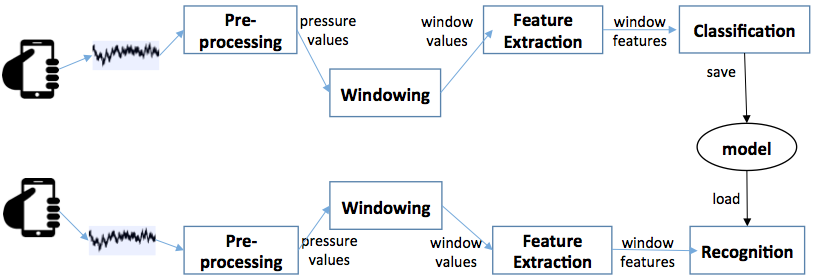
\includegraphics[width=.45\textwidth]{Block_Design_ahmad.png}
}
\caption{Design of REACH}
\label{fig:Design of REACH}
\end{figure}

The design of REACH involves three distinct phases - building the hardware to collect and transmit force sensor data, performing off-line analysis to train a classification model and finally performing real-time evaluations to detect grip patterns and perform a corresponding action. The overall design of REACH is illustrated in Figure \ref{fig:Design of REACH}.
\par
The built-in force sensors continuously send force values to the classification phase of the system. In classification phase, the force values are windowed and suitable features from the window values are extracted. These features are then used to find a suitable classification model and the parameters of the model are saved. In recognition phase, the saved classification model is used to detect the corresponding actions on the phone. We describe each phase of REACH in details in the following sections.

	% Overall Design
\section{Hardware design of REACH}
	% HW Design
\section{Software Design of REACH}
In addition to the hardware implementation by selecting appropriate force sensors and locating them in the appropriate places around the mobile device, we also build the classifier for the hand grip. In this section, we discuss how we collect force sensor values from mobile device for training and how we implement the classifier for grip pattern detection. We then used the model to predict the pattern in realtime manner.
\par
For training the model,  we used the Weka (Witten \& Frank 2005) machine learning library for Java. We used Bayesian network, Support vector machine and Classification tree algorithms for training the model on the collected data. We performed off-line training on a laptop and extracted the parameters of the best model to implement the realtime version of REACH.

\subsection{Tap Detection as Proxy}
While waiting for the hardware to be completed, we decided to perform some experiments to provide insight into how to  classify the grip patterns. Tap detection was chosen as a proxy for grip pattern detection. We used the accelerometer data available from an Android phone to try and classify instances when a user performs a single tap on the back of the device.
\par
The accelerometer data from 3 axis (x, y, z) is analogous to the force data available from the 16 sensors for grip detection. Similarly, both accelerometer and force data will change when an action is performed by the user. The only difference is that the accelerometer data changes depending on the orientation of the phone, while the force data is unaffected. To mitigate this, all data collected and analyzed for tap detection focused on keeping the phone in portrait orientation, the y-axis facing away from the floor and the z-axis facing towards the user.

\subsubsection{Determine Window Size}
The Android sensor collects accelerometer data on a periodic basis. This sampling interval is neither guaranteed nor specified by the Android SDK, but using the default mode, it was found to be 20ms on \textit{average}. After analyzing the data, it was noticed that the characteristic pattern of a single tap lasted for a duration of 400ms on average. This duration is defined as the \textit{window duration}.
\par
Dividing the window duration by the sampling interval gives us a \textit{window size} of 20. The accelerometer data is partitioned into windows with the specifications above, and implemented as a \textit{sliding window}. This means that the starting time for each subsequent window differs by the sampling interval. Contrast this against a \textit{jumping window}, where the start time for subsequent windows would be the window duration. Using the \textit{sliding window} protocol ensures that a possible tap is not missed during the evaluation process.
\par
Picking the right window size is crucial since it has a direct impact on the accuracy of the classification model. If the \textit{window size} is too small, then the complete characteristic pattern of a tap will not be captured, leading to incorrect classifications. However, using a window size that is too large will capture extraneous noisy data that will also reduce the classification accuracy. This topic will again be explored for grip pattern detection.

\subsubsection{Determine Features}
Upon observing the data, it was noticed that acceleration values of the x, y and z axis all changed when the tap action was performed. The \textit{inter}-window change was captured by calculating the \textit{mean} for a window, and this was used as one of the features for training the model. There was a visible change in the acceleration values within the window duration, and this \textit{intra}-window change was represented by calculating the \textit{variance} of a window.

\subsubsection{Classify a Tap}
Even though a windowing principle was used, windows clustered near a tap duration all show a similar characteristic pattern, albeit time-shifted. Therefore while performing the manual classification of the training data, we decided to label, on average, 20 windows as a single tap. This means that when a tap is being evaluated with real-time data, we would expect 20 back-to-back windows all to be predicted as a tap. Once such a scenario is detected, we would report a successful tap as being detected.

\subsubsection{Tap Model Performance}
We collected acceleration values of the x, y, and z dimension of three different activities on the mobile: \emph{None}, \emph{Motion}, and \emph{Tap}. The mean and variance of each window for each dimension is then calculated and are used as instance features for training a model. The Motion activity is added to represent the boundary between Tap and None activities.  The corresponding activity of each window is labeled manually (\emph{i.e.}, None, Motion, and Tap) and used as class feature for training a model. 
\par
We used Bayesian network, Naive bayes and Support vector machine algorithms with Weka's default configuration for training. We also used different number of instances with different ratios between class features. In all cases, Bayesian network was the winner among other algorithms. Table \ref{tbl-Confusion Matrix} shows the confusion matrix of using Bayesian network algorithm with 10-fold cross validation of 2250 instances (among them are 1000 None, 1000 Motion, and 250 None instances). The matrix shows that 76 of Tap activities are classified as Motion which is reasonable due to the similarity between these two activities. While 142 of Motion activities are classified as None, we believe that these are the instances which exist in the boundaries between Motion and None activities.

\begin{table}[!t]
\begin{center}
\caption{Confusion Matrix using Bayesian network with 10-fold cross validation}
\label{tbl-Confusion Matrix}
\begin{tabular}{|l||l|l|l|}\hline
        & None   & Motion   & Tap   \\ \hline \hline
None    & 970    &	29      & 1	    \\
Motion  & 142    &	825     & 33    \\
Tap     & 1      &	76      & 173	\\ \hline
\end{tabular}
\end{center}
\end{table}

\subsection{Grip Classifier}
We used the insights gained from tap detection to guide our grip classification process, namely a sliding window evaluation protocol and similar features to describe a grip pattern. We begin by attempting to classify three grip patterns in our prototype: None, Squeeze, and Reach. In None, the subject holds the device without performing any activity. In Squeeze, the subject is applying a squeeze-force on the device and in Reach, the subject is moving his thumb finger to reach the top of the device while holding the device.  
\par
The 12 force sensors around the device continuously reported data every 1 ms on average. Based on our experience with tap detection, we felt that these values could be safely aggregated into a 20ms sampling interval for the purpose of grip detection. Figure \ref{fig:window_60} shows the change in a sensors value for a \textit{window size} of 60. We can clearly see that choosing a value of 20 would result in the loss of essential information, while a value of 60 would admit noisy data. It was determined that a \textit{window size} of 50 represents the average case.

\begin{figure}[h]
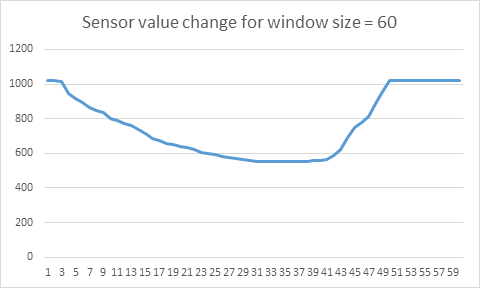
\includegraphics[width=.45\textwidth]{window_60.png}
\caption{Sensor value changes for window size 60}
\label{fig:window_60}
\end{figure}

\par
Similar to tap detection, we calculated the mean and variance for each \textit{sliding window}. It was observed that different people perform the same gesture in slightly different ways. To increase the robustness of the trained model, we decided to use the mean values of all the sensors located on one side of the device. The variance for each sensor was calculated with respect to these averaged means. For each window the following features were calculated -\textit{mean left}, \textit{mean right} and \textit{variance} for each sensor.

\subsubsection{Variability of Grip Patterns}
We wanted to establish a good baseline performance for grip pattern detection, which led us to collect all training and evaluation data from 1 subject. The individual was asked to perform Hold, Squeeze and Reach every 15 seconds for a duration of 1 minute. Each dataset collected involved repeating this process  3 times. We noticed that even for the same individual, subsequent datasets resulted in a variability of the grip patterns. The model that was trained for the first dataset performed poorly for the second dataset. However, when the second dataset was used to train the model, cross-validation performance was very similar to the original dataset. We will explore the performance further in the Evaluation section.  

	% SW Design
\section{Evaluation}
Our initial goal of having the grip classification being performed in real-time on the device was abandoned due to time constraints. Therefore we focused our evaluation criteria on how accurately the grip patterns could be identified. While training the model, we performed a 10-fold cross-validation that provides insight into the model's performance. 

\subsection{Model Evaluation}
Table \ref{tbl-Grip Model Eval} demonstrates shows the performance of the model when trained with two datasets, and two algorithms - SMO and BayesNet. As expected the prediction accuracy when a larger dataset is used. However, it should also result in a more robust model since the larger dataset contains slightly different reach gestures.
This indicates that the presence of a large training dataset should result in the robustness 

\begin{table}[!t]
\caption{Grip model cross validation accuracy with multiple datasets}
\label{tbl-Grip Model Eval}
\begin{tabular}{lllllll}
        & \multicolumn{3}{c}{initial dataset} & \multicolumn{3}{c}{expanded dataset} \\
        & count     & SVM        & Bayes      & count     & SVM        & Bayes    \\
None    & 13751     & 99.4\%     & 98.8\%     & 20773     & 99.6\%     & 99.1\%      \\
Squeeze & 871       & 97.0\%     & 99.7\%     & 871       & 95.5\%     & 97.5\%      \\
Reach   & 679       & 97.9\%     & 99.3\%     & 1361      & 94.0\%     & 95.6\%     
\end{tabular}
\end{table}

It was determined that the best performance achieved by a model for the expanded dataset was using the J48 tree classifier, as shown in  Table \ref{tbl-Grip Model J48}

\begin{table}[!t]
\caption{J48 Grip model cross-validation Confusion Matrix}
\label{tbl-Grip Model J48}
\begin{tabular}{|l|l|l|l|l|l|}
\hline
        & total & None  & Squeeze & Reach & Correct \\ \hline
None    & 20773 & 20729 & 9       & 35    & 99.8\%  \\ \hline
Squeeze & 871   & 9     & 855     & 7     & 98.2\%  \\ \hline
Reach   & 1361  & 16    & 4       & 1341  & 98.5\%  \\ \hline
\end{tabular}
\end{table}


\subsection{Off-line Evaluation}
We decided to use the J48 tree grip detection model since it produced the best cross-validation results. Since we are not performing real-time evaluation, we first record our evaluation dataset in a similar manner to the training dataset - generating a log of the sensor values as the user performs the squeeze and reach gestures. This dataset is then parsed to generate the sliding windows and extract the features. 
\par
We wrote a simple Java program running on a laptop that would load the J48 grip classification model, read the features of each window and ask the model to classify it as None, Squeeze or Reach gesture. Without looking at the predictions for each window, we classified each window manually. The accuracy of the 
			% Evaluation
\section{Conclusions and Future Works}

The initial goal of REACH was to detect a specific grip type and perform an action as result. Although we were not able to implement it in an end-to-end manner, we believe that we have demonstrated the feasibility of such a system. It is impressive to see that the classification tree machine learning algorithm was able to accurately distinguish between 3 types of grip patterns.

\par
For future work, the following key areas were identified - 
\begin{itemize}
  \item From a hardware perspective, we would like to be able to shrink the entire setup into a case for the mobile device.
  
  \item Interface with the case over a Bluetooth connection to collect the force sensor data. This data would then dynamically be windowed, the features extracted and the model would make a prediction, all in real-time on the phone.
  
  \item Collect a larger training dataset with the grip gestures being performed by multiple users. Explore other features that could lead to better predictions.
  
  \item Create a user interaction scheme that dynamically responds to the grip gestures and evaluate its effectiveness.

\end{itemize}			% Conclusions


%\end{document}  % This is where a 'short' article might terminate



%=============================================================================
% BIBLIOGRAPHY
%=============================================================================

% The following two commands are all you need in the
% initial runs of your .tex file to
% produce the bibliography for the citations in your paper.
\bibliographystyle{abbrv}
\bibliography{sigproc}  % sigproc.bib is the name of the Bibliography in this case
% You must have a proper ".bib" file
%  and remember to run:
% latex bibtex latex latex
% to resolve all references
%
% ACM needs 'a single self-contained file'!
%
%APPENDICES are optional
%\balancecolumns

\end{document}
